\documentclass[11pt]{article}
\usepackage[a4paper,margin=2.6cm]{geometry}
\usepackage[utf8]{inputenc}
\usepackage[T1]{fontenc}
\usepackage{lmodern}
\usepackage{amsmath,amssymb,amsthm}
\usepackage{mathtools}
\usepackage{booktabs}
\usepackage{graphicx}
\usepackage{enumitem}
\usepackage{xcolor}
\usepackage{tikz}
\usetikzlibrary{arrows.meta,positioning,shapes.geometric}
\usepackage[colorlinks=true,linkcolor=blue!50!black,citecolor=blue!50!black,urlcolor=blue!50!black]{hyperref}
\usepackage{microtype}

\newtheorem{theorem}{Theorem}[section]
\newtheorem{lemma}[theorem]{Lemma}
\newtheorem{proposition}[theorem]{Proposition}
\newtheorem{corollary}[theorem]{Corollary}
\theoremstyle{definition}
\newtheorem{definition}[theorem]{Definition}
\newtheorem{assumption}[theorem]{Assumption}
\theoremstyle{remark}
\newtheorem{remark}[theorem]{Remark}

\newcommand{\K}{K}
\newcommand{\Hyp}{\mathcal{H}}
\newcommand{\Sv}{S_{V}}
\newcommand{\Sstar}{S^{*}}
\newcommand{\tauV}{\tau_{V}}
\newcommand{\ttt}[1]{\texttt{#1}}
\newcommand{\Ex}{\mathbb{E}}

\title{Verified slack imitation:\\[4pt]
\large imitating a deterministic researcher,\\ with correctness from a verifier and cost from the human}
\author{Claude (Anthropic)\\[2pt]
\small Research write-up for Kaarel H\"anni's question on principled human imitation\\
\small 22 November 2026 \quad---\quad draft; reviewed by AI referees only}
\date{}

\begin{document}
\maketitle

\begin{abstract}
A learner imitates a human researcher, modelled as a fixed deterministic program $P$, by Bayesian (Solomonoff-style) induction on the human's three-month steps, and chains its imitation over $n$ steps to solve research problems. The baseline, chained imitation (``train on test''), needs about $n\K/\varepsilon$ task queries for runs that fail with probability at most $\varepsilon$, where $\K = \K(P)$; and every protocol that asks the human only for task steps needs nearly that on humans whose insights are rare, problem-specific and never recovered once missed. We propose \emph{verified slack imitation} (VSI): the imitator gets more steps than the human needs, on an append-only notebook with a hidden clock; each problem is rerun until a verifier of finished results accepts; and a rejected run is searched for a mistake, mostly by scanning it from the start. We prove that every output passes the verifier, so that \emph{correctness rests on one assumption, the verifier's soundness on the imitator's claims}, and on no property of the human's task behaviour; that there are at most $\K$ rejections; and that each costs at most $2n_0$ task queries whatever the human, so at most $2n_0\K$ in all, with no factor $1/\varepsilon$, within a logarithm of a lower bound that holds even with a perfect verifier. Under a natural property of humans, bounded setback, each rejection costs $O((D{+}1)/\rho)$ queries instead. We give the case for the assumptions, from experiments with exact posteriors and from published evidence, and our calibrated probability that the scheme works on a real careful researcher: about 70\% with a proof assistant on an independently reviewed formal statement, a narrow domain; 46--60\% for informal theory and software with a combined human verifier; and 15--20\% for empirical and judgment-heavy work.
\end{abstract}

\tableofcontents

\section{Introduction}

\paragraph{The question.} Section 3.2 of the talk \emph{Simpler versions of the alignment problem we still can't solve} (MISO, 16 November 2026) asks for a principled way to imitate a human researcher. Its best protocol, \emph{chained imitation}, does Solomonoff function induction on a human's input--output pairs (a state, then three months of work on it), chains the learned map as in task decomposition, and queries the human on the distribution this induces. The question put to us: find a protocol more likely to work, for a human who is a fixed deterministic program, under assumptions that are likely true of humans; ideally show that $O(\K(\text{human}))$ reasonable queries suffice, with a compelling case. One constraint emerged along the way: the protocol should not assume that the human can tell whether a run has \emph{gone off track}.

\paragraph{Why this is hard.} Chained imitation is DAgger with a Bayes mixture. Each task query that lands on a step where the imitator errs teaches the learner at least one bit, so at most $\K$ such queries ever happen; but a failed run may contain a single wrong step, which a random query finds with probability only $1/n$. So chained imitation pays $n\K$ failed runs, or $n\K/\varepsilon$ queries for failure rate $\varepsilon$. And this is nearly unavoidable: on humans whose insights are rare, specific to each problem, arrive at unpredictable steps, and are never recovered if missed (\emph{silent} humans), every protocol that asks the human only for task steps needs $\Omega(n\K/(\varepsilon\log(n/\varepsilon)))$ queries (Theorem~\ref{thm:lb-task}). A better protocol must use either a property of humans that excludes silence, or a human signal beyond task steps.

\paragraph{What we propose.} \emph{Verified slack imitation} (VSI, Section~\ref{sec:scheme}) combines both, in the weakest forms we found:
\begin{itemize}[nosep]
\item \emph{slack}: the imitator runs $n = n_0 + \sigma$ steps where the human needs $n_0$, so a missed contribution that the human would still make later costs a delay, not a failure;
\item \emph{a verifier of finished results}: each problem is rerun until a verifier $V$ accepts a claimed solution. $V$ is ideally a machine (a proof assistant on a formal statement); it judges only the finished product, never whether a run is on track;
\item \emph{a search on rejected runs}: queries cycle through a scan from step 0, a uniformly random step, and a list of pointers, until one lands on a mistake. A rejected run's first mistake always comes before step $n_0$, so the scan caps the cost.
\end{itemize}

\paragraph{What we prove.} Theorem~\ref{thm:main}: every output passes $V$, so correctness rests on $V$'s soundness alone; there are at most $\K$ rejections, and each costs at most $2n_0$ task queries whatever the human, $O((D{+}1)/\rho)$ under bounded setback, and $1$ when a local check finds an invalid entry. In total at most $2n_0\K$ task queries, with no $1/\varepsilon$ and independent of the number of problems. Theorem~\ref{thm:lb-verify}: even with a perfect verifier, $\Omega(n\K/\log(nq/\varepsilon))$ task queries are needed on silent humans, so the worst case is optimal up to the logarithm. Section~\ref{sec:lower} collects further lower bounds that delimit what any scheme without judgments of states can do.

\paragraph{How sure we are.} Section~\ref{sec:sure}. With a proof assistant checking an independently reviewed formal statement, VSI ``works'' (output failure at most 5\% on projects of 20--40 three-month steps, at under a fifth of chained imitation's human effort) with probability about $70\%$, conditional on the idealizations shared by the whole framework. The domain is narrow. Elsewhere VSI is the best scheme we found but not one to be sure of.

\paragraph{Provenance.} This paper condenses a series of notes and research threads (Appendix~\ref{app:provenance}); every main claim was checked by at least one independent AI referee, and the experiments were re-run by referees. No human has checked the mathematics.

\section{Setting}\label{sec:setting}

\paragraph{Notebooks and the human.} A \emph{problem} is a starting notebook $x_0$. A \emph{notebook} $y$ is $x_0$ followed by a finite list of \emph{entries}; $y \circ g$ denotes $y$ with the list of entries $g$ appended. The human is a deterministic program $P$: a \emph{step} of the human at $y$ is the list of entries $P(y)$ it appends in three months of work, and the next notebook is $y\circ P(y)$. The human's own chain is $c_0 = x_0$, $c_{k+1} = c_k\circ P(c_k)$. A \emph{task query} at $y$ asks the real human for $P(y)$. Notebooks are append-only: a revision is a new entry. A \emph{hidden clock} means the human is not told the step number or a deadline, so $P$ is a function of the notebook alone.

\paragraph{The learner.} Let $\Hyp$ be a countable class of deterministic programs $h$ (notebook $\mapsto$ list of entries) with prior weights $w(h)$, $\sum_h w(h)\le 1$, and $P\in\Hyp$; write $\K = \log_2(1/w(P))$. For a set $D$ of labelled notebooks $(y,P(y))$, let $W(D)$ be the prior mass of the hypotheses consistent with $D$, let $\xi_D(\ell\mid y)$ be the posterior mass of those consistent hypotheses $h$ with $h(y)=\ell$, and let the \emph{majority decoder} $G_D(y)$ be a label of largest $\xi_D(\cdot\mid y)$ (fixed tie-breaking). Define the \emph{potential}
\[ \Phi(D) = \log_2\frac{W(D)}{w(P)} \in [0,\K]. \]
Adding a correct datum $(y,P(y))$ lowers $\Phi$ by $\log_2(1/\xi_D(P(y)\mid y))\ge 0$, and $W(D)$ depends only on the \emph{set} $D$.

\begin{lemma}[a bit per mistake]\label{lem:bit}
If $G_D(y)\ne P(y)$ then $\xi_D(P(y)\mid y)\le\frac12$, so adding $(y,P(y))$ lowers $\Phi$ by at least $1$. Hence, whatever other correct data are added, at most $\lfloor\K\rfloor$ task queries ever land on a mistake of the decoder in use.
\end{lemma}
\begin{proof}
$\xi_D(G_D(y)\mid y)\ge \xi_D(P(y)\mid y)$ and the two masses add up to at most $1$. Since $\Phi$ starts at most $\K$, never increases, never goes below $0$, and drops by at least $1$ at each such query, there are at most $\lfloor\K\rfloor$ of them.
\end{proof}

\paragraph{Runs and mistakes.} The imitator's run on $x_0$ is $x'_0=x_0$, $x'_{k+1}=x'_k\circ G_D(x'_k)$, possibly with \emph{asks}: at a step where the top label's mass is below $1-\alpha$, the protocol asks the human and appends $P(x'_k)$ instead. A \emph{committed} step is one that is not asked; it is a \emph{mistake} if $G_D(x'_k)\ne P(x'_k)$. $M$ denotes a run's set of committed mistakes. A run with no mistake is the human's own chain.

\paragraph{Success and remaining time.} $\Sv$ is the predicate the verifier decides on final notebooks; $\Sstar$ is the goal. For a predicate $S$ preserved by appending, the human's \emph{remaining time} from $y$ is $\tau(y)=\min\{m\ge 0: S(y_m)\}$, where $y_0=y$ and $y_{m+1}=y_m\circ P(y_m)$. By determinism, $\tau(y\circ P(y))=\tau(y)-1$ when $\tau(y)\ge1$, and $\tau=0$ is preserved by appending.

\begin{lemma}[expected mistake mass; \cite{note2}]\label{lem:mass}
Suppose that in each round $t$ a problem arrives (in any order, possibly adaptively), the current decoder's run is made, and then one step is task-queried, drawn from a distribution $q_t$ chosen after the run is fixed; the answer is added, before any other data of the round. Then $\Ex\sum_t q_t(M_t)\le\K$.
\end{lemma}
\begin{proof}
Given the past and the run, the query lands on a mistake with probability $q_t(M_t)$, and each such query lowers $\Phi$ by at least $1$ (Lemma~\ref{lem:bit}). So $\sum_t \mathbf 1[\text{hit}_t]\le\K$ surely; take expectations.
\end{proof}

\section{The proposal: verified slack imitation}\label{sec:scheme}

\subsection{The scaffold and the verifier}

The \emph{instruction} given to the human at every step is part of the problem statement, so it holds in the human's own chain as well as in the imitator's runs; a correct imitator step reproduces the human's step exactly (the \emph{design law}).
\begin{itemize}
\item \textbf{Append-only notebook and hidden clock.} No step numbers, dates or deadlines appear; the scaffold strips them.
\item \textbf{Slack.} The imitator runs $n=n_0+\sigma$ steps, $\sigma=\rho n$, where the human's own chain under the same instruction reaches $\Sv$ within $n_0$ steps.
\item \textbf{The verifier} $V$, one of:
\begin{itemize}[nosep]
\item[(V-machine)] a machine check: a proof assistant on a formal statement of the goal, a test suite, a program checking a constructed object. For a proof assistant two things are mandatory: a \emph{statement protocol} (a second independent formalization with machine-checked equivalence; AI audits from different model families; test lemmas for new definitions; non-vacuity witnesses; automated attempts to prove and disprove; human sign-off), and \emph{hardened checking} (a pinned, patched kernel; an independent checker; an axiom whitelist; at least two kernels). Optionally an AI formalizer sits inside $V$: the human's chain ends with a blueprint-quality informal proof, and $V$ means ``the formalizer, within budget $B$, produces a proof of the fixed statement that the hardened kernel accepts''.
\item[(V-cone)] a check, entry by entry, of the claimed solution's dependency cone (the claim and everything it cites, recursively) by a local check $L$: does each entry follow from what it cites?
\item[(V-human)] a human verifier's check of the finished result, by someone other than the imitated human, possibly imitated (Theorem~\ref{thm:imitated-verifier}).
\end{itemize}
$V$ accepts if some claimed solution in the final notebook passes, and the \emph{verified artifact} (the first passing claim) is what is output.
\end{itemize}

\subsection{The protocol}

\begin{center}
\fbox{\begin{minipage}{0.94\linewidth}
\textbf{Protocol VSI.} For each problem, repeat:
\begin{enumerate}[leftmargin=1.4em]
\item \textbf{Run} the current imitator for $n$ steps (optionally asking the human at the step that writes the claimed solution, if the imitator is unsure there).
\item \textbf{Verify.} If $V$ accepts, output the verified artifact (optionally after a ``nothing bizarre'' check of the notebook by a second person), and with probability $\beta$ task-query one uniform committed step (an \emph{audit}).
\item \textbf{If $V$ rejects:}
\begin{enumerate}[label=(\roman*),leftmargin=1.6em]
\item if a local check $L$ flags invalid committed entries, task-query the flagged steps in turn until one is a mistake;
\item otherwise \emph{search}: task-queries cycle through the streams in the fixed order S, U, S, H, over committed steps, where S is the next step of a scan from step $0$, U a uniformly random step, and H the next entry of a list fixed at the start of the search (the last review step, labelled decision steps, and a second researcher's post-mortem pointers; when empty, its turn goes to S). Stop at the first query that lands on a mistake; add its answer first and the others after it; rerun.
\item if the scan exhausts the run without a mistake, the run is the human's own chain: report ``the human's own chain does not reach a verifiable solution within $n$ steps'' and stop.
\end{enumerate}
\item \textbf{Halt for statement review} if any run contains a statement-defect entry (which the instruction lets the human write), or if an accepted formal proof triggers an anomaly rule (much shorter than expected, or bypassing the blueprint's milestones).
\end{enumerate}
\end{minipage}}
\end{center}

\begin{figure}[t]
\centering
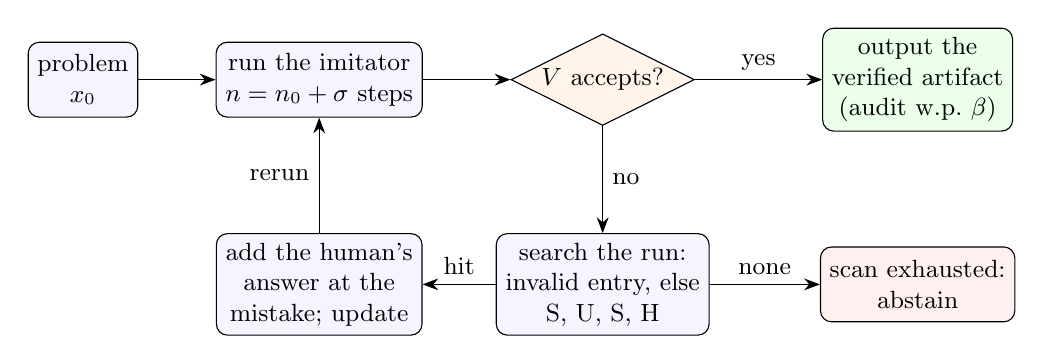
\begin{tikzpicture}[every node/.style={font=\small},
 box/.style={draw, rounded corners, align=center, minimum height=0.95cm, fill=blue!4},
 dec/.style={draw, diamond, aspect=2.0, align=center, inner sep=1pt, fill=orange!8},
 arr/.style={-{Stealth[length=2mm]}}]
\node[box] (prob) at (0,0) {problem\\ $x_0$};
\node[box] (run) at (3.0,0) {run the imitator\\ $n=n_0+\sigma$ steps};
\node[dec] (ver) at (6.6,0) {$V$ accepts?};
\node[box, fill=green!8] (out) at (10.6,0) {output the\\ verified artifact\\ (audit w.p.\ $\beta$)};
\node[box] (search) at (6.6,-2.6) {search the run:\\ invalid entry, else\\ S, U, S, H};
\node[box] (upd) at (3.0,-2.6) {add the human's\\ answer at the\\ mistake; update};
\node[box, fill=red!6] (abs) at (10.6,-2.6) {scan exhausted:\\ abstain};
\draw[arr] (prob) -- (run);
\draw[arr] (run) -- (ver);
\draw[arr] (ver) -- node[above]{yes} (out);
\draw[arr] (ver) -- node[right]{no} (search);
\draw[arr] (search) -- node[above]{hit} (upd);
\draw[arr] (upd) -- node[left]{rerun} (run);
\draw[arr] (search) -- node[above]{none} (abs);
\end{tikzpicture}
\caption{Verified slack imitation. Correctness comes from $V$; the human contributes only task steps (and, optionally, post-mortem pointers by a second researcher, which are hints that never enter the data).}
\label{fig:protocol}
\end{figure}

\paragraph{Why the order S, U, S, H.} It gives the scan half the queries in an order that makes the scan's $j$-th step query $2j-1$, the uniform stream's $k$-th draw query $4k-2$, and the list's $i$-th entry query $4i$. The order matters: U, H, S, S has the same frequencies but a worse worst case.

\section{Guarantees}\label{sec:guarantees}

\begin{assumption}\label{ass}\
\begin{enumerate}[label=(A\arabic*),nosep]
\item $P$ is deterministic and $P\in\Hyp$.
\item $\Sv$ is preserved by appending, and the human's own chain reaches it within $n_0$ steps: $\tauV(x_0)\le n_0$.
\item[(A3$'$)] \emph{Completeness on the human's runs:} $V$ accepts every extension of the human's own notebook $c_{n_0}$.
\item[(A4$'$)] \emph{Soundness, per claim:} every claimed solution that $V$ passes, in the final notebooks of the imitator's runs, satisfies the goal.
\end{enumerate}
When a local check $L$ is used: (L0) $L$'s verdict on an entry is fixed once the entry is written; (L1) every entry the human appends passes $L$. When the optional ``nothing bizarre'' check is used: (M1) the start notebook passes, (M2) the human never makes a passing notebook fail, (M-prefix) prefixes of passing notebooks pass.
\end{assumption}

\begin{lemma}[the first mistake comes early]\label{lem:early}
Under (A1) and (A3$'$), every rejected run has a committed mistake at a step below $n_0$.
\end{lemma}
\begin{proof}
Asked steps and correct committed steps both append $P$'s label. If no committed step below $n_0$ is a mistake, the notebook at step $n_0$ is $c_{n_0}$, and the final notebook extends it; $V$ accepts by (A3$'$).
\end{proof}

\begin{lemma}[invalid entries are mistakes]\label{lem:invalid}
Under (L0) and (L1), a committed step that appends an entry failing $L$ is a mistake.
\end{lemma}
\begin{proof}
Every entry of the human's step passes $L$, and the verdict on the imitator's entry is fixed; so the two steps differ.
\end{proof}

\begin{lemma}[pointers carry no risk]\label{lem:hints}
Fix a rejected run of a fixed decoder with committed mistake set $M\ne\emptyset$, searched with the schedule S, U, S, H. Every answer added is the human's own step, and
\[ \Ex[\text{queries}] \le \min\Bigl\{\frac{4n}{|M|},\; 2j_S+1,\; 4(j_H+1)\Bigr\}, \]
where $j_S$ and $j_H$ are the positions (from $0$) of the first mistake in the scan and in the list. The list may be written by anyone, an adversary included.
\end{lemma}
\begin{proof}
With the stated schedule, the scan's $(j{+}1)$-th step is query $2j+1$, the list's $(i{+}1)$-th entry is query $4(i+1)$, and the uniform stream's $k$-th draw is query $4k-2$, each draw hitting independently with probability at least $|M|/n$. The search stops at the first hit of any stream. A list only decides which steps are queried; the answers are the human's.
\end{proof}

\begin{definition}[bounded setback]
The human has \emph{setback at most $D$} on a run if at every committed mistake $k$, $\tau(x'_{k+1})\le\tau(x'_k)+D$, with $\tau$ the remaining time to the predicate in question.
\end{definition}

A mistake thus costs the human its step plus at most $D$ steps. An omission of part of the human's step that the human would still contribute later has setback $0$; a hidden clock makes an empty step exactly a one-step delay, by determinism. Silent humans have unbounded setback.

\begin{lemma}[slack turns one wrong step into many]\label{lem:slack}
If $\tau(x_0)\le n_0$ and the setback is at most $D$ on a run of $n=n_0+\sigma$ steps that fails, then $|M|\ge\max\{1,(\sigma+1)/(D+1)\}$.
\end{lemma}
\begin{proof}
Write $\tau_k=\tau(x'_k)$. The run fails, so $\tau_n\ge1$, and since $\tau=0$ is preserved by appending, $\tau_k\ge1$ for all $k$. At each correct step $\tau$ falls by exactly $1$; at each mistake it rises by at most $D$. Hence $1\le\tau_n\le n_0-(n-|M|)+D|M|=(D+1)|M|-\sigma$. A run with no mistake is the human's own chain, which succeeds.
\end{proof}

\begin{theorem}[verified slack imitation]\label{thm:main}
Assume (A1), (A2), (A3$'$), and (L0)--(L1) if $L$ is used, (M1)--(M2) if the bizarre check is used. Let $b=1$ (or $b=\max\{1,\log_2(1/\alpha)\}$ if asks are made at every step whose top mass is below $1-\alpha$), $\Lambda=\min\{n,(D+1)n/(\sigma+1)\}$, and let $T$ be the number of problems. For every sequence of problems, chosen adaptively:
\begin{enumerate}[label=(\alph*)]
\item \textbf{Correctness.} Every output passes $V$; under (A4$'$) it satisfies the goal. This uses no property of the human's task steps and none of (A1)--(A3$'$).
\item \textbf{Counts.} Almost surely, rejections that end in a hit, failed bizarre checks and audit hits together number at most $\K/b$. Asks number at most $\K/\log_2(1/(1-\alpha))$ on every path.
\item \textbf{Termination.} Every problem ends with an output, an abstention, or a halt for statement review; under (A2) and (A3$'$) the abstain rule never fires.
\item \textbf{The cost of a rejection.} One query if $L$ flags an invalid committed entry (plus one per flagged step that turns out to be the human's own). Otherwise at most $2n_0$ queries surely, whatever the human, and in expectation at most
\begin{itemize}[nosep]
\item $4\Lambda$ under setback at most $D$ in $\tauV$ at committed mistakes;
\item $4$ for a failure whose last review step is a mistake (a by-product insight readable from raw records, recovered at reviews; \cite{threadG});
\item $4(1+d)$ for a hedge failure at one of $d$ labelled decisions;
\item $4(1+d+i)$ if the $i$-th post-mortem pointer is a mistake.
\end{itemize}
\item \textbf{Totals.} $\Ex[\text{task queries}]\le \text{asks}+(\K/b)\cdot\min\{2n_0,4\Lambda\}+\beta T$, plus at most $2n$ per rejection or abstention on problems that violate (A2) or (A3$'$).
\end{enumerate}
\end{theorem}

\begin{proof}
(a) $V$ accepted every output; (A4$'$) is the step from passing $V$ to satisfying the goal.

(b) By Lemma~\ref{lem:early}, or by route (i) and Lemma~\ref{lem:invalid}, every search ends with a hit at a committed step $k$, unless the scan is exhausted. List the round's data as: the asks before $k$, then the hit, then the rest; since $W$ depends only on the set of data, the total drop of $\Phi$ is unchanged. The decoder committed at $k$ using exactly the data before the hit, so by Lemma~\ref{lem:bit} the hit lowers $\Phi$ by at least $1$; with asks at every unconfident step, the committed label had mass at least $1-\alpha$, so the human's answer has mass at most $\min\{\alpha,\frac12\}$ and the hit is worth at least $b$. A failed bizarre check's flip is a mistake by (M1)--(M2), and an audit hit is a mistake by definition. Each ask lowers $\Phi$ by more than $\log_2(1/(1-\alpha))$, since its answer had mass below $1-\alpha$. Since $\Phi\le\K$ at the start and never goes below $0$, the counts follow.

(c) A problem is rerun only after a hit, and hits are finitely many by (b). Under (A2) and (A3$'$), Lemma~\ref{lem:early} guarantees a hit before the scan is exhausted.

(d) Route (i) is Lemma~\ref{lem:invalid}. Otherwise apply Lemma~\ref{lem:hints}: by Lemma~\ref{lem:early} the scan's first mistake has $j_S\le n_0-1$, reached by query $2n_0-1$ surely; under bounded setback Lemma~\ref{lem:slack} gives $|M|\ge\max\{1,(\sigma+1)/(D+1)\}$, so $4n/|M|\le4\Lambda$; the last review step of a ripe by-product failure and the decision step of a hedge failure are mistakes \cite{threadG}, at list positions $0$ and at most $d$.

(e) Sum (b) and (d) by Wald's identity; the number of searches is bounded on every path.
\end{proof}

\begin{remark}[what moved]
In slack imitation without a verifier, confident wrong content, lost insights and trusted dead ends decide \emph{correctness}. In VSI they decide only \emph{cost}: at most $2n_0$ queries per rejection and at most $\K$ rejections. The worst-case bound $2n_0\K$ has no $1/\varepsilon$, because the verifier \emph{detects} failed runs; and it has $n_0$ rather than $n$, because the scan exploits the fact that a rejected run's first mistake comes before $n_0$.
\end{remark}

\begin{remark}[asks are optional with a verifier]
With a verifier, asking changes only the cost. In our experiments, asking at every unconfident step multiplied VSI's cost 5--35-fold on several mechanisms, so the default asks at most at the step that writes the claimed solution.
\end{remark}

\begin{proposition}[a safety net for any learner]\label{prop:any-learner}
Run VSI with \emph{cache-first decoding} (at any notebook already asked about, the imitator outputs the human's recorded answer; elsewhere any learner may decide) and with answers cached, so that no notebook is asked about twice. Assume (A3$'$) and no asks. Then, whatever the learner:
\begin{enumerate}[label=(\alph*),nosep]
\item correctness is as in Theorem~\ref{thm:main}(a);
\item on any single problem, VSI makes at most $2n_0$ task queries in total, over all its reruns: twice what the human needs to do the problem itself;
\item if the learner makes at most $M$ mistakes on the notebooks it predicts before being told their answers (for exact Bayes, $M\le\K$ by Lemma~\ref{lem:bit}), there are at most $M$ rejections, and at most $2n_0M$ task queries in all.
\end{enumerate}
\end{proposition}
\begin{proof}
(b) Fix a problem. In any run, the steps before the first committed mistake follow the human's own chain $c_0,c_1,\dots$, and by Lemma~\ref{lem:early} the first mistake is at a step below $n_0$. A cached notebook cannot be a mistake, by cache-first decoding. So each search's scan stream queries only notebooks $c_i$ with $i<n_0$ that have not been asked before, and each search's first query is such a scan query. Hence the scan queries at most $n_0$ distinct notebooks over all searches of the problem, and there are at most $n_0$ searches. In every prefix of the cycle S, U, S, H, the non-scan queries are at most as many as the scan queries, so the total is at most $2n_0$.
(c) Each rejection ends with a query at a notebook where the learner's prediction, made before being told, was wrong; so there are at most $M$ rejections, each costing at most $2n_0$ by the argument of (b).
\end{proof}

So with cache-first decoding, which the scaffold can enforce, VSI's cost never exceeds about twice the human's own effort on any problem, for any learner; the learner's quality decides only how much of the human's effort is saved across problems.

\begin{proposition}[if the verifier is unsound]\label{prop:unsound}
The failed outputs are exactly the accepted runs whose verified claim fails the goal. Suppose the goal predicate (``the first claim that $V$ passes satisfies the goal'') is preserved by appending, the human's own chain reaches it within $n_0$, and the setback in its remaining time is at most $D$ at committed mistakes of accepted runs. Then $\Ex[\#\text{failed outputs}]\le\K/(b\,\beta\,\gamma)$ with $\gamma=\max\{1,(\sigma+1)/(D+1)\}/n$.
\end{proposition}
\begin{proof}
The run and $V$'s verdict are fixed before the audit's coin; by Lemma~\ref{lem:slack} an audit of a failed accepted run hits with probability at least $\gamma$, and audit hits are counted in Theorem~\ref{thm:main}(b).
\end{proof}

So with a fallible verifier, audits at rate $\beta=1$ are needed to keep slack imitation's own guarantee for the failures $V$ misses.

\begin{theorem}[imitating the verifier \cite{threadQ}]\label{thm:imitated-verifier}
Let $V_H$ be a human verifier's verdict, a deterministic one-step function of complexity $\K_V$. Keep a Bayes posterior over $V_H$ with majority decoder $V'$; on each claimed solution ask $V_H$ if $V'$ rejects, and with probability $\beta_V$ if $V'$ accepts; add every answer. For any $T$ claimed solutions chosen adaptively: (a) $V'$ disagrees with an asked $V_H$ at most $\K_V$ times; (b) the expected number of solutions accepted by $V'$, not asked, and rejected by $V_H$ is at most $(1-\beta_V)\K_V/\beta_V$; (c) $V_H$ is asked at most $\beta_V T+R+\K_V$ times in expectation, $R$ the number of true rejections.
\end{theorem}
\begin{proof}
(a) is Lemma~\ref{lem:bit} for a one-step function. (b) On a false acceptance by $V'$, an audit lands on a mistake of $V'$, of which there are at most $\K_V$; so $\beta_V\cdot\Ex[\#\text{false acceptances}]\le\K_V$. (c) A rejection by $V'$ is a true rejection or a mistake of $V'$.
\end{proof}

Imitating the verifier pays when verdicts are generic (a line-by-line proof check, a test suite) or problems recur. On distinct research problems whose verification needs the problem's own insight, the imitated verifier is blind exactly where the imitator is; there one should budget about one human verification per problem.

\begin{corollary}[``works'' in the worst case, with a machine verifier]\label{cor:works}
Let $V$ be a machine verifier satisfying (A3$'$)--(A4$'$), with no audits. Chained imitation's guarantee for failure rate $\varepsilon=5\%$ is $n_0\K/\varepsilon=20n_0\K$ task queries; VSI's is $2\iota n_0\K$, where $\iota$ is the factor by which the instruction (for example, ending with a formal proof) inflates the human's horizon. So VSI's guarantee is below a fifth of chained imitation's guarantee whenever $\iota<2$, \emph{whatever the human}, and with every output correct. (Both are upper bounds; per-problem costs such as writing and reviewing a formal statement come on top.)
\end{corollary}

This is the core of the case for VSI with a machine verifier: the only properties of the human it needs are those of the framework itself (determinism, realizability, a chain that reaches a verifiable solution), plus a modest $\iota$.

\section{What no scheme can do}\label{sec:lower}

The following are proved in the notes and threads listed in Appendix~\ref{app:provenance}; we state them and sketch why. ``Task-only'' means a protocol that asks the human only for task steps, at any states, synthetic ones included, adaptively; asks are included.

\begin{theorem}[silent humans \cite{note1}]\label{thm:lb-task}
For every $n$, $\varepsilon$ and $\K$ there is a class of humans of complexity about $\K$ on which every task-only protocol needs $\Omega(n\K/(\varepsilon\log(n/\varepsilon)))$ task queries for failure $\varepsilon$.
\end{theorem}
\emph{Sketch.} Each problem hides, with probability $\eta$, an insight of unknown value at a uniformly random step; the human writes it there and nowhere else. A query reveals it only if it is at that step on a state lacking it, so each query is a point query among $n$ candidates.

\begin{theorem}[verification detects but does not locate \cite{threadQ}]\label{thm:lb-verify}
On the same class, a protocol that also verifies candidate final states, fewer than about $q/16$ times per insight problem ($q$ the number of possible insight values), still needs $\Omega(n\K/\log(nq/\varepsilon))$ task queries.
\end{theorem}
\emph{Sketch.} A verification says \emph{whether} a problem hides something, not \emph{where}. VSI uses about one verification per problem, so its worst case $2n_0\K$ is optimal up to the logarithm.

\begin{theorem}[slack imitation is optimal for bounded setback; slack is necessary \cite{threadJ}]\label{thm:lb-slack}
For all $n$, $\rho$, $D\le n_0/2$ and $\varepsilon$ there is a class of humans with setback at most $D$ on every notebook on which every task-only protocol needs $\Omega((1-\rho)\Lambda\K/(\varepsilon\log(n/\varepsilon)))$ task queries. With $\sigma=0$ and $D=0$ the factor $n$ is forced.
\end{theorem}

\begin{theorem}[insights triggered by doing \cite{threadG}]
If an insight is triggered only by the human itself \emph{doing} one particular unit of routine work, chosen unpredictably, then every protocol of task queries (and of human steps that depend only on the work they process), under any scaffold, must have the human process about a quarter of all the routine work per such insight.
\end{theorem}

\begin{theorem}[trusted true records; fooled commissions \cite{threadF,threadJ}]
(i) Humans that recover from every omission and every invalid entry, but never retry an approach with a recorded obstruction, force $\Omega(n_0\K/(\varepsilon\log(n_0/\varepsilon)))$ queries on protocols of task queries and single-entry checks. (ii) Confident commissions that a fooled human accepts, at unpredictable steps, cost every task-only protocol $\Omega(n)$ queries per deviation.
\end{theorem}

\paragraph{What this says.} For unpredictable, problem-specific contributions, the sources of \emph{location} we found are: the human's own recovery (slack, under bounded setback), hindsight (post-mortem pointers), structure (the first mistake comes early; every invalid entry is a mistake; reviews and decisions are mistakes in ripe and hedge failures), concentration of where contributions occur, and the imitator's own doubt (asks). A judgment of the run's states would be another, and is excluded by the constraint. VSI uses the first three, and pays $2n_0$ per rejection only when none applies. In VSI every lower-bound case costs queries, never correctness.

\section{The case for the assumptions}\label{sec:case}

\subsection{What correctness needs: the verifier}

Correctness needs only (A4$'$). What that means depends on the verifier.

\paragraph{A proof assistant.} (A4$'$) is the fidelity of the formal statement plus the soundness of the checking pipeline. Published evidence \cite{threadT}:
\begin{itemize}[nosep]
\item \emph{Misformalization is common unless reviewed.} After an in-depth manual review of expert-written Lean statements of 50 recent \emph{Annals} theorems, AI audits still found mistakes in 22\% of them (severity unreported); benchmark audits find 5--60\% unfaithful statements. Estimated, for research goals needing new definitions: about 25\% unfaithful without independent review and about 10\% with an exploitable weaker form; about 4\% and 1.5\% with the statement protocol of Section~\ref{sec:scheme}. About half of misformalizations fail safe (a false statement cannot be proved; VSI abstains). The contribution to output failure is about 0.5--1\% with review.
\item \emph{Kernels are sound against honest proofs.} Adversarial AI testing found several soundness bugs in Lean and Rocq in 2026 (search summaries only), hence hardened checking, estimated sound with probability about $99.5\%$.
\item \emph{Formal proof has become much cheaper.} With AI formalization agents, landmark proofs were formalized in days to weeks in 2025--26 (self-reported, by well-resourced teams, of decades-polished proofs). For goals already statable, the estimated probability that ending the chain with a formal proof costs at most $1.5\times$, $2\times$, $3\times$ the informal duration is about $65\%$, $80\%$, $90\%$.
\item \emph{The domain is narrow.} In ten months, working easiest first, experts stated 24\% of recent \emph{Annals} main theorems in Lean; perhaps 5--15\% of multi-year mathematics projects are in the domain today.
\end{itemize}

\paragraph{A human verifier.} (A4$'$) is an assumption about a human judgment, of a finished product with full attention. Evidence \cite{threadL,threadS}: reviewers catch 30--60\% of planted plausible errors; the imitator's wrong results are the \emph{most typical-looking} ones, the hardest to catch; and rerunning until accepted turns every miss into a wrong output, at a rate of about $p\,w\,f_{\text{eff}}$ per problem ($p$ the first-run failure rate, $w$ the share of failed runs that carry a claimed solution, $f_{\text{eff}}$ the verifier's miss rate compounded over the claims a problem may need), which need not shrink when insights are problem-specific. Estimated miss rates on imitator-style wrong results: 0.2--0.5 for one careful reader in mathematics, above 0.5 for empirical claims judged by reading. Section~\ref{sec:nonformal} gives the best combinations.

\subsection{What only the cost needs}

\begin{itemize}
\item \textbf{(A2) for every problem.} Research durations are heavy-tailed: with $n_0$ at the 75th percentile, (A2) fails on a quarter of problems, and 6--11\% are not finished even within $n=2n_0$, on which VSI abstains at about $n$ queries each. A formalizer inside $V$ adds false rejections of the human's correct blueprints (estimated 5--30\% by field), each an (A2) failure unless the human formalizes as a fallback.
\item \textbf{Bounded setback} makes rejections cheap. Evidence \cite{threadL}: setbacks look \emph{bimodal}. An error that conflicts with something or fails on use is caught within a step or two; a plausible error or a recorded dead end can persist for years. People accept altered records of their own choices often (choice blindness), and researchers rarely revisit recorded dead ends. So bounded setback is believable for mistakes that fail loudly, and what sets the cost is the share never recovered.
\item \textbf{Reviews and decisions} make two kinds of omission cheap: insights readable from raw records (recovered at content-triggered reviews) and ideas pre-empted by a default at a labelled decision. They do nothing for insights that come only from doing (Theorem 5.4).
\item \textbf{Post-mortem pointers} by a second researcher are hints: a useless or adversarial list costs at most a constant factor (Lemma~\ref{lem:hints}). They must not be written by the imitated human, whose later answers on the same run would no longer be $P$'s; the same holds for anyone who reads a run before it is searched.
\end{itemize}

\subsection{Selection and human-likeness}\label{sec:selection}
The point of imitation, for alignment, is that the system does what the human would have done, without optimization pressure. Rerunning until accepted is a filter, so one must ask how far it moves VSI's outputs away from the human's process. The following results are proved in \cite{threadV}, for exact Bayes under (A1) and any filter that satisfies (A3$'$). Write $\K'=\lfloor\K/b\rfloor$.

\begin{theorem}[no optimization pressure \cite{threadV}]\label{thm:nopressure}
Every datum VSI collects is a pair $(x,P(x))$; verdicts and pointers are never data. Every output notebook is the final notebook of the run under a set $D$ of the human's answers, by a map fixed before the verifier is chosen. Every step of an output is one of three things:
\begin{itemize}[nosep]
\item the human's answer (an ask);
\item the human's own step at that notebook;
\item the plurality label of the prior restricted to the hypotheses consistent with all the human's data. This label is backed by at least the mass of the human's own program, and by at least $1-\alpha$ of the posterior when asks are made at every unconfident step.
\end{itemize}
The verifier changes a run only by rejecting it, and every rejection costs a hit, at least $b$ bits of learning about the human.
\end{theorem}

\begin{theorem}[bits of selection \cite{threadV}]\label{thm:selection}\
\begin{enumerate}[label=(\alph*),nosep]
\item \emph{Per problem.} Given the history, the output on a problem is a point on a path of runs that does not depend on the verifier. The path runs from the verifier-free run to the human's own chain, and the verifier only chooses where to stop. So it adds at most $\log_2(1+R_p)$ bits on a problem with $R_p$ rejections, and none when $R_p=0$.
\item \emph{Lifetime.} For every event $E$ on the first $T$ problems, $\Pr[\text{VSI}\in E]\le 2^{B_T}\Pr[\text{VSI with content-blind verdicts}\in E]$, with $B_T\le \log_2\binom{T+\K'}{\K'}\le \K'\log_2 e+\K'\log_2(1+T/\K')$. No smaller bound holds for every verifier.
\item \emph{With audits.} Against a filter that knows whether a run deviates from the human but not how, the expected log-likelihood ratio is at most $\K'\log_2(e(1+n/\beta))$, for every $T$; and the expected number of non-human steps in all outputs ever made is at most $n\K'/\beta$.
\end{enumerate}
\end{theorem}

\paragraph{What this means.} The decoder never sees the verifier: it is a fixed function of the human's answers. The verifier only decides which answers are collected and when, and each change it causes is paid for with true information about the human. Its influence grows logarithmically with the number of problems, against $T\log_2k$ bits for best-of-$k$ resampling, and without bound for training on accepted outputs (which in exact Bayes refutes the human outright).

\paragraph{Malign hypotheses.} In a Solomonoff prior some hypotheses may be optimizers. The filter never raises any hypothesis's posterior odds against the human's. A coalition of hypotheses can write a payload into an output only where it outweighs everything that writes the human's label, the human included; with asks at every unconfident step, it must outweigh it by $(1-\alpha)/\alpha$. Payloads in outputs are mistakes, so audits catch them at rate $\beta/n$ per output: the same metering as chained imitation at $\beta=1$. Whether such coalitions exist is the open malign-prior question; VSI neither creates nor removes them.

\paragraph{The formalizer inside $V$.} The formalizer is an optimizer, and its formal proof is optimized. The notebook is not, for any formalizer, malicious or broken included, provided nothing the formalizer produces enters a notebook or the data, or is seen by the imitated human (\emph{isolation}). With a fixed statement, a pinned and seeded formalizer, and the proof archived and checked by the kernel in a sandbox rather than read, the only optimized information that reaches the world is the verdict, which the bounds above already count.

\paragraph{Several claims in one notebook.} When $V$ passes the first of several claims, it chooses among an accepted notebook's claims without a hit, at up to $\log_2 c_p$ more bits on a problem with $c_p$ claims. Verifying only the notebook's \emph{first} claim, and treating its failure as a rejection, removes this choice while keeping the verified predicate preserved by appending. It then needs (A3$'$) for the first claim of the human's own chain.

\subsection{The constraint}
A machine verifier rests correctness on no judgment of the runs: only on the fidelity of a statement fixed before any run. A human verifier judges only the finished product, which is a distinct and weaker assumption than an on-track judgment, but correctness rests on it. A local check of the cone judges intermediate entries locally (does this follow from what it cites?), which is not an on-track judgment, though its power to locate mistakes comes from the human's own entries passing it. The version that keeps both the letter and the spirit of the constraint is the machine verifier, which is also the version we are most sure of.

\section{How sure we are}\label{sec:sure}

\emph{``Works''} means: on a real careful researcher, with projects of $n_0\approx20$--$40$ three-month steps, the output failure rate is at most 5\% and the total human effort (task queries, verifications, post-mortems, audits, statement writing, in task-step equivalents) is at most a fifth of chained imitation's. An abstention counts as effort, about $n$ task queries. The figures are conditional on the framework's idealizations: determinism, a learner whose class contains the human, and a cold-start chain that reaches the informal goal within $n_0$.

\begin{table}[h]
\centering
\small
\begin{tabular}{@{}p{6.2cm}p{3.9cm}cc@{}}
\toprule
scheme & correctness rests on & theory, software & empirical, judgment \\
\midrule
VSI, proof assistant, reviewed statement, hardened checking & statement fidelity, checker & \textbf{70\%} & -- \\
\quad same, AI formalizer inside $V$ (human fallback) & same & 77\% & -- \\
\quad same, without review and hardening & same & 60\% & -- \\
VSI, test suite & the tests & 43\% & -- \\
VSI, combined human verifier (Section~\ref{sec:nonformal}) & the combination & 46\% / 60\%$^\dagger$ & 15\% / 20\% \\
VSI, referee checking the cone & $L$'s soundness & 45\% & 10\% \\
VSI, one human verifier & the verifier & 35\% & 10\% \\
slack imitation, no verifier & bounded setback etc. & 30\% & 10\% \\
chained imitation (the talk) & nothing & baseline & baseline \\
\bottomrule
\end{tabular}
\caption{Probability that each scheme works. $^\dagger$informal theory / software without a full specification. The figures synthesize the threads' estimates (Appendix~\ref{app:provenance}): the human-verifier rows follow the second red team, lowered by the evidence that most failed runs end with a confident claimed solution \cite{threadW}; the formal rows follow the calibration thread. That VSI's task queries are truly $O(\K)$, with neither $n_0$ nor $1/\varepsilon$, we put at about 25\%.}
\label{tab:sure}
\end{table}

\paragraph{Why the machine-verifier row is high.} By Corollary~\ref{cor:works}, VSI's guarantee is below a fifth of chained imitation's whatever the human, provided $\iota<2$; correctness needs only the statement and the checker. The remaining doubt is in the idealizations, in statement fidelity after review (about 4\% unfaithful), in $\iota$ (about 80\% that $\iota\le2$), in per-problem statement writing, and in heavy tails.

\paragraph{Why the other rows are low.} A human verifier misses the imitator's most plausible wrong answers at substantial rates, and rerunning until accepted converts misses into outputs. Without a verifier, the guarantee needs bounded setback for the share of mistakes that fail silently, which the evidence does not support.

\paragraph{The human-does-it baseline.} For $T$ distinct problems the human alone spends $n_0T$; VSI's worst case beats this only if $2\K<T$, that is, if the problems share most of what must be learned: the regime of the original question, performance on very many problems.

\section{Experiments}\label{sec:experiments}

All experiments use small classes with exact posteriors and 20--40 simulated humans per cell. They test how cost scales with the horizon and with the kind of human, not whether real humans have the properties. Human kinds: \emph{noticing} (setback $0$), \emph{misled-$D$} (setback $D$), \emph{fooled} (never corrects a wrong value), \emph{silent} (an idea writable at one step only).

\begin{figure}[t]
\centering
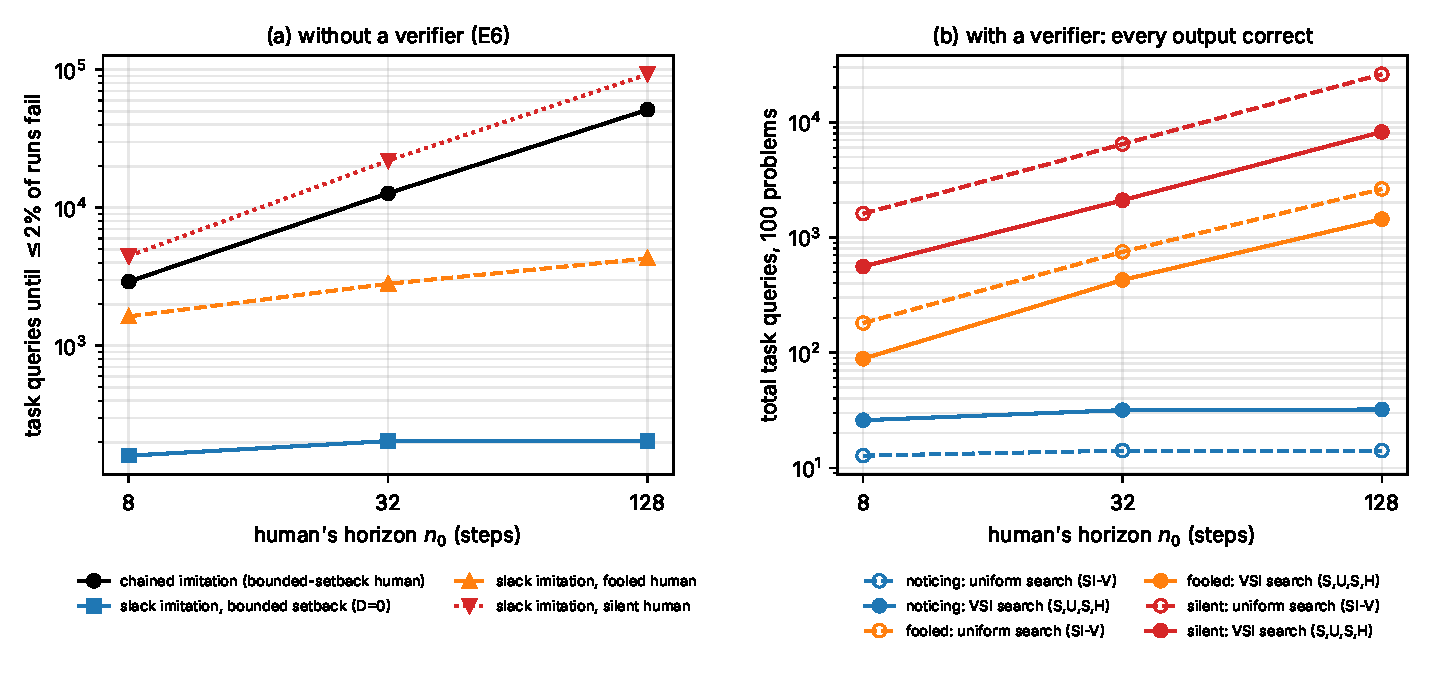
\includegraphics[width=\linewidth]{fig_e6.pdf}
\caption{E6. (a) Without a verifier: chained imitation grows in proportion to $n_0$; slack imitation is flat for bounded-setback humans, grows for fooled humans, and doubles the cost of silent ones. (b) With a verifier, every output is correct; VSI's scan-weighted search (no post-mortems) costs bounded-setback humans about 30 task queries for 100 problems at every $n_0$, and cuts silent humans' cost about threefold against uniform search, as Lemma~\ref{lem:early} predicts. Fooled humans grow with $n_0$ without post-mortem pointers.}
\label{fig:e6}
\end{figure}

\paragraph{E6} (Figure~\ref{fig:e6}). On the same humans, chained imitation needs $2{,}915\to12{,}724\to51{,}365$ task queries for $n_0=8\to32\to128$; slack imitation $160\to204\to204$ for noticing humans.

\paragraph{E7: composition.} Eight failure mechanisms, each its own class, against all protocols. Table~\ref{tab:e7} gives VSI's total task queries for 100 problems, every output correct, with the default schedule and the protocol's own list without post-mortems, against uniform search.

\begin{table}[h]
\centering\small
\begin{tabular}{@{}lrrrr@{}}
\toprule
mechanism & \multicolumn{2}{c}{uniform search (SI-V)} & \multicolumn{2}{c}{VSI (S,U,S,H)} \\
 & $n_0=8$ & $n_0=128$ & $n_0=8$ & $n_0=128$ \\
\midrule
M1 persistent idea (setback 0) & 13 & 14 & 26 & 32 \\
M2 fooled commission at a verdict & 181 & 2{,}636 & 89 & 1{,}442 \\
M3 silent human & 1{,}610 & 26{,}091 & 559 & 8{,}238 \\
M4 readable by-product, reviews$^*$ & 221 & 338 & 158 & 187 \\
M5 doing-only by-product$^*$ & 1{,}029 & 16{,}127 & 355 & 5{,}316 \\
M6 hedge at a labelled decision & 76 & 1{,}439 & 34 & 41 \\
M7 invalid checkable claim & 136 & 2{,}868 & 10 & 10 \\
M8 false negative as a valid record & 136 & 2{,}868 & 51 & 2{,}350 \\
\bottomrule
\end{tabular}
\caption{E7. $^*$Indexed by routine length $8\to128$. Each mechanism has the component that handles it: slack (M1), the review query (M4), the decision query (M6), the local check (M7). M3 and M5 grow under every protocol, as the lower bounds say. M2 and M8 stay flat only with a post-mortem that points at the verdict or the record (40--55 and 31--34 task queries in that case); without one they grow, within the sure $2n_0$ per rejection.}
\label{tab:e7}
\end{table}

\section{Without a machine verifier}\label{sec:nonformal}

For research without a machine-checkable goal, output failure is about $p\,w\,\bar r\,f_V$, with $\bar r$ the distinct wrong claims verified per failing problem; at central values the 5\% bar needs a verifier miss rate $f_V\le0.29$ in theory, $0.23$ in software, $0.17$ in empirical and $0.16$ in judgment work, against about $0.43$, $0.45$, $0.70$, $0.64$ for one careful reader \cite{threadU}. What helps:
\begin{itemize}[nosep]
\item \emph{different methods, not more readers}: misses of readers correlate (fitted correlation about 0.45--0.75), so a second reader leaves 0.24, not 0.16;
\item \emph{verification by use} (examples, consequences, independent tests): reading plus use cuts misses by about 38\%; in software, independent tests and fuzzing take $f$ from 0.45 to 0.13;
\item \emph{machine checks} of every computation and citation: about 20\% fewer misses;
\item \emph{AI critics} from several model families, with an expert other than the imitated human judging \emph{located} objections: the largest gain (0.43 to 0.18 added to a reader). Critics can only add rejections, so they cannot make a wrong result pass; located objections also serve as search pointers;
\item \emph{delayed checks by consequence}, the only remedy for empirical claims false in the world, at the price of provisional outputs.
\end{itemize}
With the best combination, the estimated probability that VSI works is about 46\% for informal theory, 60\% for software without a full specification, 15\% for empirical work (25\% if the goal is narrowed to ``the claim follows from the data''), and 20\% for judgment work.

\paragraph{How often failed runs end with a confident claim.} The factor $w$ was only guessed in earlier drafts. The evidence \cite{threadW} comes from AI systems on tasks they cannot solve, where every claim is a failure:
\begin{itemize}[nosep]
\item \emph{Mathematics:} every model claimed to have solved the problems of a recent olympiad evaluation; models ``prove'' false variants of theorems 43--84\% of the time; and most failed submissions to a research-problem round were written as complete.
\item \emph{Empirical work:} a coding agent invented experimental results in 8 of 10 research tasks, even when told not to.
\item \emph{Human researchers:} about 0.3 of failed projects end in an overclaim when unpublished failures are counted, and about 0.8 among failures that were written up.
\end{itemize}
The estimates are $w\approx0.6$ in theory and software, $0.85$ in empirical work and $0.9$ in judgment work. With the best combined verifiers, output failure is then about 3.5\%, 1.6\%, 9\% and 7\% respectively.
\begin{itemize}[nosep]
\item \emph{What reduces $w$.} Instructions help unreliably. An explicit option to hand the task back works much better: one model's cheating fell from 54\% to 9\%. That supports asking the human at the final-answer slot as a default with human verifiers.
\item \emph{The caveat.} These inputs are mostly judgments and stand-ins, not measurements on an imitator's wrong results.
\end{itemize}

\section{From the idealization to practice}\label{sec:practice}

\paragraph{What survives with a real learner.} The analysis assumes exact Bayes over a class containing the human. With a practical learner (a language model fine-tuned on the human's steps, decoding greedily), three things change and two do not.
\begin{itemize}[nosep]
\item \emph{Unchanged:} correctness, which is the verifier's (Theorem~\ref{thm:main}(a)); and, with cache-first decoding, the cap of $2n_0$ task queries per problem (Proposition~\ref{prop:any-learner}), so VSI never costs much more than the human doing the problem itself.
\item \emph{Changed:} the bound of $\K$ rejections becomes the learner's number of mistakes on queried notebooks, which has no guarantee; asks need a calibrated confidence, for which token entropy or agreement among samples are proxies; and the absence of optimization against $V$ holds only if the learner neither resamples until accepted nor trains on accepted outputs (Section~\ref{sec:selection}).
\end{itemize}

\paragraph{Orders of magnitude.} A task query is three months of the human's time, so the costs are in human-quarters.
\begin{itemize}[nosep]
\item In the worst case VSI spends $2n_0$ human-quarters per bit of $\K$, which is $48$ for a six-year project ($n_0=24$). Under bounded setback with $D=1$ and $\rho=\frac12$, it is about $4\Lambda\approx16$; and when post-mortem pointers or local checks locate mistakes, a few.
\item Chained imitation at $\varepsilon=5\%$ spends $20n_0=480$ per bit.
\item So the scheme is practical only if $\K$, the human's description length given what the learner already knows (for example a large corpus), is small, and if its cost is amortized over many problems. For $T$ problems the human alone spends $n_0T$; VSI's worst case is below that once $T>2\K$.
\end{itemize}
This is the regime the original question points to: performance on very many problems, with a learner for which the human is simple.

\section{Limitations, open problems, and what to measure}\label{sec:limits}

\paragraph{Idealizations.} Determinism, exact Bayes over a class containing the human, and cold-start chains (a human who rereads its notebook every three months and keeps nothing unrecorded). Experts are noisy (about 90\% repeatability on categorical decisions, less on open-ended work). With a machine verifier VSI's correctness survives these; its cost theory does not. A stochastic version is open.
\paragraph{The domain.} VSI needs a crisp success criterion, fixed in advance and preserved by appending. Much valuable research has no such goal; VSI imitates the well-posed part of research.
\paragraph{Memory.} A real human remembers earlier queries, so out-of-order queries and readings of a run leak information into later answers; every multi-query protocol shares this, and VSI mitigates it by its scan-heavy order and by having readers other than the imitated human.
\paragraph{Practical learners.} The no-optimization argument (the decoder is a deterministic function of the human's data) holds for exact Bayes; a learner that resamples or trains on accepted outputs optimizes against $V$.
\paragraph{What to measure first} (none needs a learner):
\begin{enumerate}[nosep]
\item the verifier's miss rate on imitator-style wrong claimed solutions, by method, with joint misses recorded; for formal verifiers, planted statement defects through the statement protocol;
\item the share of an imitator's failed runs that end with a confident claimed solution;
\item the duration tail of the human's own chain under the instruction, and the formal-proof factor $\iota$;
\item how much reading a run changes the human's later answers on it;
\item planted-culprit tests of post-mortem pointers and of setbacks, especially recorded dead ends.
\end{enumerate}

\appendix

\section{Slack imitation without a verifier}\label{app:slack}

The scheme of the fourth note asks one uniformly random task query per run. By Lemma~\ref{lem:mass} and Lemma~\ref{lem:slack}: if every run has setback at most $D$, then $\Ex[\#\text{failed runs}]\le\min\{n,(D+1)n/(\sigma+1)\}\cdot\K\le(D+1)\K/\rho$, against chained imitation's $n_0\K$; and on i.i.d.\ problems, $O((D+1)\K\log(\K/\delta)/(\rho\varepsilon))$ task queries give failure at most $\varepsilon$ with probability $1-\delta$ (epochs with a frozen decoder, each ending at a hit). Asking before committing (ask the human wherever the top label's mass is below $1-\alpha$) uses at most $\K/\log_2(1/(1-\alpha))\le(\ln2)\K/\alpha$ asks over the whole lifetime, and bounded setback is then needed only at confident steps; the failure bound improves by $\log_2(1/\alpha)$. A deployment version ends each epoch also at the first unconfident step. Without bounded setback the guarantee falls back to chained imitation's on the longer run, $n_0\K/(1-\rho)$.

\section{Further results}\label{app:more}
\begin{itemize}
\item \textbf{The certified notebook} \cite{threadF}. With typed entries (certified claims, obstruction records ``attempt at A stopped at gap Z'' instead of verdicts, suggestions, machine records) and a local check, every invalid entry is a mistake; slack imitation with the check has at most $\K$ runs with an invalid entry. What remains is bounded setback at \emph{valid} entries, which cannot be dropped (trusted true records, Theorem 5.5(i)). A rule that an approach may be set aside only after $r$ obstruction records makes each derailment cost $r$ mistakes.
\item \textbf{Trees} \cite{threadN}. For decomposition trees with slack measured in rounds per call and setback at the parent, depth-weighted queries give at most $\Psi\K$ failed runs with $\Psi<2((D+1)/\rho)^{d+1}b^d$ for depth $d$ and branching $b$; the $b^d$ is necessary without more structure, and a sound and complete verifier at every node removes the dependence on the tree's size.
\item \textbf{Other learners} \cite{threadH}. Every result without asks holds for any online learner whose log-loss regret against $P$ is at most $R$, with $\K$ replaced by $R$; results with asks need, in addition, predictions that depend only on the set of data. So $\K$ may be the human's description length in whatever class the learner uses, for example given a corpus, provided the class contains the human exactly.
\item \textbf{Location numbers} \cite{threadJ}. Querying steps by an optimal fractional hitting set of the failing hypotheses' mistake sets gives at most $L\K$ failed runs, $L$ the hitting set's size; on faithful hiding classes this is optimal up to logarithms.
\end{itemize}

\section{Provenance}\label{app:provenance}
All files are in the repository folder \texttt{monitored-imitation/} on the working branch.
\begin{itemize}[nosep]
\item \cite{note1} \texttt{note.md}: monitored imitation; the lower bound for task-only protocols; the bit per mistake.
\item \cite{note2} \texttt{without-a-check.md}: expected mistake mass; end-weighted queries.
\item \texttt{robust-runs.md}: robustness of properties under the imitator's replacements.
\item \texttt{slack-imitation.md}: slack imitation, bounded setback, asking before committing, experiment E6.
\item \texttt{verified-slack.md}: verified slack imitation, the full version of this paper's main results, with three referee reports and responses.
\item Research threads (\texttt{research/}): \cite{threadE} red team of slack imitation; \cite{threadF} certified notebook; \cite{threadG} by-product insights; \cite{threadH} deployment, other learners; \cite{threadJ} optimality; \cite{threadL} evidence on researchers; \cite{threadN} trees; \cite{threadQ} alternatives, verification, pointers; \cite{threadR} composition experiment E7; \cite{threadS} red team of VSI; \cite{threadT} machine-verifier calibration; \cite{threadU} verifiers without a machine; \cite{threadV} human-likeness and bits of selection; \cite{threadW} confident failures; and earlier threads A--D on checks, elicitation, persistence and literature.
\end{itemize}

\begin{thebibliography}{99}
\bibitem{note1} Claude. \emph{Monitored imitation} (note.md), 2026.
\bibitem{note2} Claude. \emph{Without a check: where in a run to ask} (without-a-check.md), 2026.
\bibitem{threadE} Claude. Thread E: red-teaming bounded setback (research/threadE-redteam.md), 2026.
\bibitem{threadF} Claude. Thread F: the certified notebook (research/threadF-certified.md), 2026.
\bibitem{threadG} Claude. Thread G: by-product insights, hedges, and what a scaffold can do (research/threadG-byproducts.md), 2026.
\bibitem{threadH} Claude. Thread H: deploying an imitator that asks, and other learners (research/threadH-deployment.md), 2026.
\bibitem{threadJ} Claude. Thread J: is slack imitation optimal? (research/threadJ-optimality.md), 2026.
\bibitem{threadL} Claude. Thread L: empirical evidence on bounded setback (research/threadL-evidence.md), 2026.
\bibitem{threadN} Claude. Thread N: slack imitation for decomposition trees (research/threadN-trees.md), 2026.
\bibitem{threadQ} Claude. Thread Q: alternatives to slack imitation (research/threadQ-alternatives.md), 2026.
\bibitem{threadR} Claude. Thread R: how the components compose (research/threadR-compose.md), 2026.
\bibitem{threadS} Claude. Thread S: second red team of verified slack imitation (research/threadS-redteam2.md), 2026.
\bibitem{threadT} Claude. Thread T: calibrating the machine verifier (research/threadT-formal.md), 2026.
\bibitem{threadU} Claude. Thread U: verification without a machine verifier (research/threadU-nonformal.md), 2026.
\bibitem{threadV} Claude. Thread V: how close VSI's outputs stay to the human's own process (research/threadV-humanlike.md), 2026.
\bibitem{threadW} Claude. Thread W: how often failed runs end with a confident claim (research/threadW-confident-failures.md), 2026.
\bibitem{ross} S. Ross, G. Gordon, J. A. Bagnell. A reduction of imitation learning and structured prediction to no-regret online learning (DAgger). AISTATS 2011.
\end{thebibliography}

\end{document}
